%%%%%%%%%%%%%%%%%%%%%%%%%%%%%%%%%%%%%%%%%
% MUW Poster
% LaTeX Template
% Version 1.0 (31/08/2016)
% (Based on Version 1.0 (31/08/2015) of the Jacobs Portrait Poster
%
% License:
% CC BY-NC-SA 3.0 (http://creativecommons.org/licenses/by-nc-sa/3.0/)
%
% Created by:
% Nicolas Ballarini, CeMSIIS, Medical University of Vienna
% nicoballarini@gmail.com
% http://statistics.msi.meduniwien.ac.at/
%%%%%%%%%%%%%%%%%%%%%%%%%%%%%%%%%%%%%%%%%


\def\footer#1{\def\insertfooter{#1}}
%--------------------------------------------------------------------------------------
%	PACKAGES AND OTHER DOCUMENT CONFIGURATIONS
%--------------------------------------------------------------------------------------

\documentclass[final]{beamer}



\usepackage[scale=1.150]{beamerposter} % Use the beamerposter package
\usetheme{MUWposter} % Use the MUWposter theme supplied with this template

% Include a logo of your project if desired
%\logo{\pgfputat{\pgfxy(-11,107)}{\pgfbox[center,base]{
\includegraphics[width=7cm]{ibga.jpg}}}}  


\usepackage{multicol}
\usepackage{array}
%The following two are column definitions for the aknowledgements section
\newcolumntype{L}{>{\arraybackslash}m{22cm}}
\newcolumntype{S}{>{\arraybackslash}m{6cm}}
\usepackage{pgf}  
\usepackage{mathtools}
\usepackage{amsmath, amsthm, amssymb, amsfonts}
\usepackage{exscale}
\usepackage{xcolor}
\usepackage{ushort}
\usepackage{setspace}
\usepackage[square,numbers]{natbib}
\usepackage{url}
\bibliographystyle{abbrvnat}
\renewcommand{\vec}[1]{\ushort{#1}}
\renewcommand{\vec}[1]{\mathbf{#1}}
\definecolor{greenMUW}{RGB}{60,191,174}
\definecolor{blueMUW}{RGB}{17,29,79}
\definecolor{skinMUW}{RGB}{254,228,217}
\definecolor{hellblauMUW}{RGB}{95,180,229}

%-----------------------------------------------
%  START Set the colors
%  Uncomment to apply colors you want to use.
%-----------------------------------------------
\colorlet{themecolor}{greenMUW}
\usebackgroundtemplate{
\includegraphics{MUW_logos.pdf}}

%\colorlet{themecolor}{skinMUW}
%\colorlet{themecolor}{blueMUW}
%\usebackgroundtemplate{
\includegraphics{MUW_skin.pdf}}

%%\colorlet{themecolor}{blueMUW}
%\colorlet{themecolor}{hellblauMUW}
%\usebackgroundtemplate{
\includegraphics{MUW_hellblau.pdf}}
%-----------------------------------------------
%  END Set the colors
%-----------------------------------------------


%-----------------------------------------------
%  START Set the width of the columns
%-----------------------------------------------
\setlength{\paperwidth}{33.1in} % A0 width: 46.8in
\setlength{\paperheight}{46.8in} % A0 height: 33.1in
\newlength{\sepmargin}
\newlength{\sepwid}
\newlength{\onecolwid}
\newlength{\twocolwid}
\newlength{\threecolwid}

% The following measures are used for 2 columns
\setlength{\sepmargin}{0.055\paperwidth} % Separation width (white space) between columns
\setlength{\sepwid}{0.03\paperwidth} % Separation width (white space) between columns
\setlength{\onecolwid}{0.43\paperwidth} % Width of one column
\setlength{\twocolwid}{0.9\paperwidth} % Width of two columns

%-----------------------------------------------------------
% The following measures are used for 3 columns
%\setlength{\sepmargin}{0.06\paperwidth} % Separation width (white space) between columns
%\setlength{\sepwid}{0.02\paperwidth} % Separation width (white space) between columns
%\setlength{\onecolwid}{0.28\paperwidth} % Width of one column
%\setlength{\twocolwid}{0.58\paperwidth} % Width of two columns
%\setlength{\threecolwid}{0.88\paperwidth} % Width of three columns
%\setlength{\columnsep}{30pt}

%-----------------------------------------------
%  END Set the width of the columns
%-----------------------------------------------


%--------------------------------------------------------------------------------------
%	TITLE SECTION 
%--------------------------------------------------------------------------------------
\setbeamertemplate{title}[left]
\setbeamertemplate{frametitle}[default][left]
%\setmainfont{Georgia}

\title{Aplicación de un índice de integridad biótica para humedales en dos lagunas urbanas pampeanas} % Poster title

\author{Valeria Jacqueline Taborda¹, Melina Celeste Crettaz Minaglia²³, Carina Apartin¹, Guillermo Sebastian Natale¹ y Alberto Rodrigues-Capítulo⁴} % Author(s)

\institute{1 Centro de Investigaciones de Medio Ambiente, CIM-UNLP-CONICET. 
2  Laboratorio de Indicadores Biológicos y Gestión Ambiental de Calidad de Agua, IBGA-FCyT-UADER.
3 Área Biología y Bioinformática, Instituto de Ciencia, UNGS.
4 Instituto de Limnología -Dr. Raúl A. Ringuelet- (ILPLA- FCNyM- UNLP-CONICET)} % Institution(s)
%--------------------------------------------------------------------------------------



\begin{document}

  \addtobeamertemplate{block end}{}{\vspace*{1ex}} % White space under blocks
  \addtobeamertemplate{block alerted end}{}{\vspace*{0ex}} % White space under highlighted (alert) blocks
  \setlength{\belowcaptionskip}{2ex} % White space under figures
  \setlength\belowdisplayshortskip{1ex} % White space under equations
  
  
  \begin{frame}[t] % The whole poster is enclosed in one beamer frame

      \begin{columns}[t] % The whole poster consists of two major columns
	  
      \begin{column}{\sepmargin}\end{column}
      
	    \begin{column}{\onecolwid} % The first column


		  \begin{block}{Introducción}
          %\begin{multicols}{2}
          Existen ambientes someros ubicados dentro de la traza urbana considerados como lagunas o humedales, que generalmente, suelen estar afectados en distinto grado por estresores ambientales. Entre las herramientas para evaluar la calidad de estos ambientes, se encuentran los índices de integridad biótica (IBI, Karr, 1986). El presente trabajo tuvo como objetivo evaluar la integridad biótica de dos lagunas urbanas a través de la aplicación de un IBI para humedales urbanos, desarrollado por  Lunde y  Resh \cite{lunde}, basado en  ensambles de macroinvertebrados acuáticos. 
          %\end{multicols}
          \end{block}
          
          \begin{block}{Metodología}
          %\begin{multicols}{2}
          Para ambas lagunas, se realizaron 3 muestreos entre el 2015-2018, de acuerdo al siguiente esquema. 
          %\end{multicols} 
          \end{block}
          
           \begin{multicols}{2}
                \begin{figure}
                	\vspace*{-0.90cm}
                    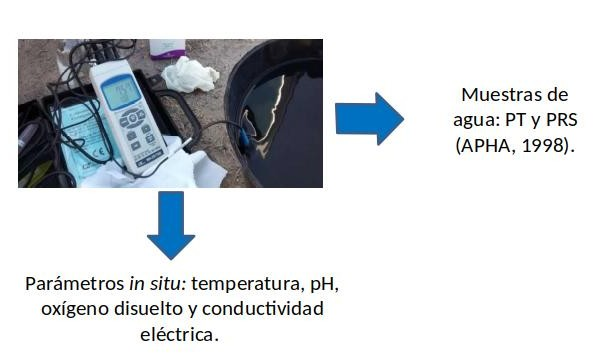
\includegraphics[width=0.9\linewidth]{met.jpg}
				\end{figure}
                \begin{figure}
                	\vspace*{-0.90cm}
                    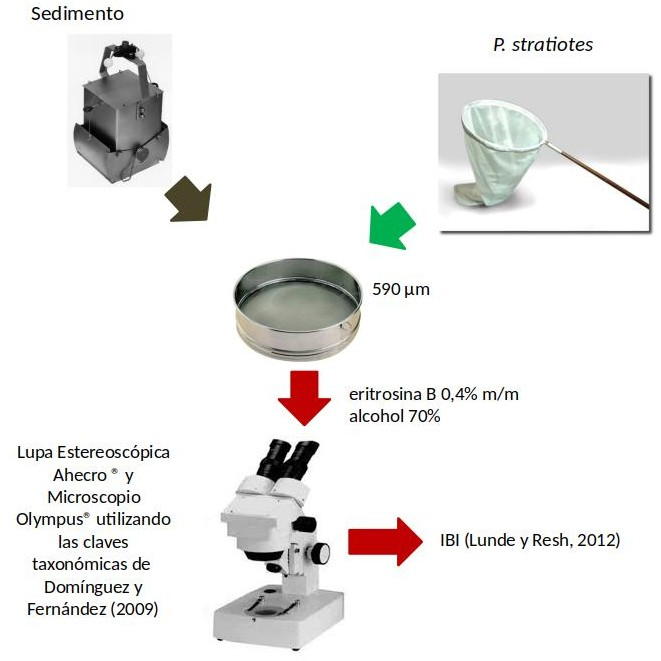
\includegraphics[width=1.1\linewidth]{met2.jpg}
				\end{figure}
                \end{multicols}
          
         % \begin{table}[ht]
		%			\centering
		%			\begin{tabular}{lccc}
         %           Patient Characteristics & n 		& & \%  %\\
		%			\hline
		%			Total of Patients 		& 100     	& & 100 %\\
		%			Age 	 				&  45      	& &  45 %\\
		%			Gender 					&  50 	   	& &  50 %\\
		%		    \hline
		%		  \end{tabular}
		%		\caption{Considered scenarios} 
         %       \label{Patient and tumor Characteristics}
		%	  \end{table}
          
          
          \begin{block}{Resultados}
          %\begin{multicols}{2}
         Los resultados obtenidos para la LPU fueron: abundancia 316 individuos y una riqueza de 14 taxones con un valor del IBI=22, mientras que para la LLP, se halló una abundancia de 3494 individuos y una riqueza de 38 taxones con un valor del IBI=80 (Tabla 1). Los resultados indican que  LPU posee una menor abundancia y riqueza taxonómica así como un valor del IBI más bajo que la LLP. En la Tabla 2, se observan los valores promedio de las variables fisico-quimicas medidas. 
         
         %\end{multicols}
          \end{block}
          
          
          \begin{block}{Conclusión}
          %\begin{multicols}{2}
          Siguiendo la interpretación propuesta por los autores del IBI, concluimos que el valor del IBI obtenido para la LPU es el esperado para sitios con alto impacto urbano mientras que la LLP presentó un valor del IBI asignado para sitios con muy poco impacto urbano, coincidiendo con la información obtenida de la prospección de las lagunas, del valor del ICR y los parámetros de calidad de agua, indicando que  la implementación del IBI resultó adecuada para estos ambientes. 
          %\end{multicols}
          \end{block}
          
         \end{column}
                  
                  
                  
         \begin{column}{\sepwid}  \end{column}
         
         
         
         
         \begin{column}{\onecolwid} %The second column
         
         %\begin{block}{\vspace*{2.7cm}}
          %%\begin{multicols}{2}
        
          %%\end{multicols}
          %\end{block}
         \begin{figure}
                  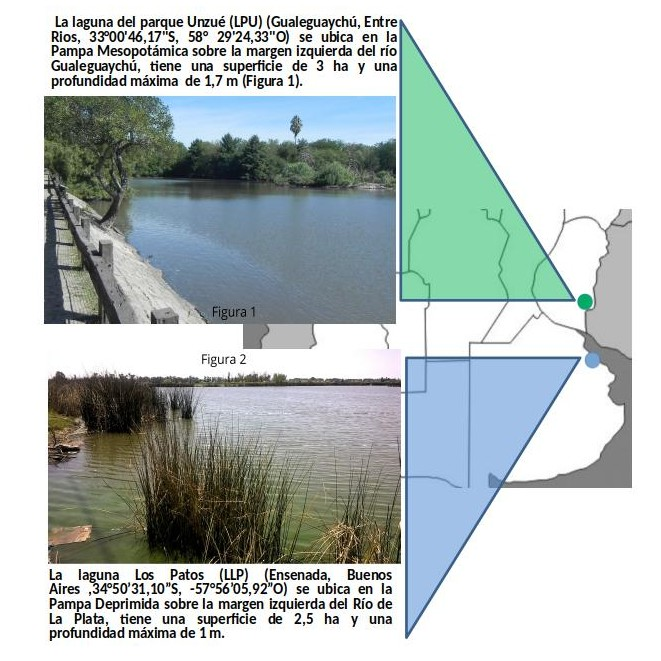
\includegraphics[width=.75\linewidth]{area_estudio.jpg}
				\end{figure}
				
				\begin{figure}
                  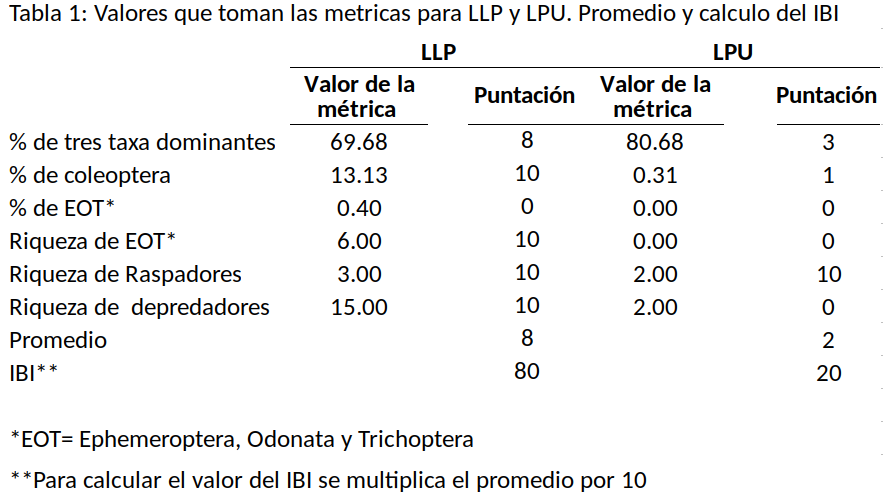
\includegraphics[width=.8\linewidth]{ibi.png}
				\end{figure}
				
				\begin{figure}
                  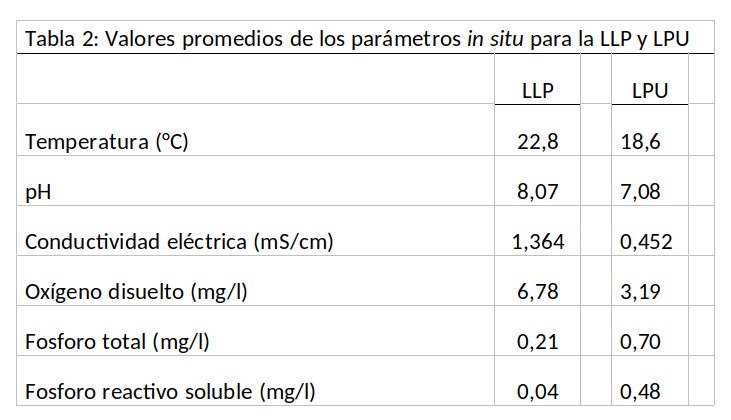
\includegraphics[width=.8\linewidth]{fq.png}
				\end{figure}
				
			
         \begin{block}{ }
			%	\begin{figure}
             %   	\vspace*{-1cm}
              %      %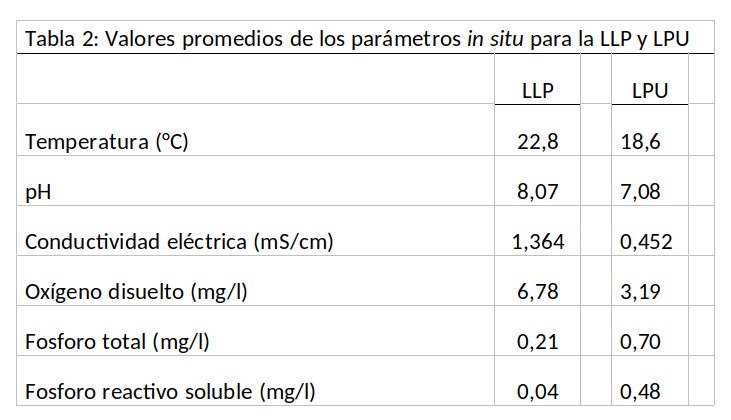
\includegraphics[width=.6\linewidth]{fq.png}
			%	\end{figure}
				%\begin{multicols}{2}
                %\begin{figure}
                %	\vspace*{-0.90cm}
                 %   %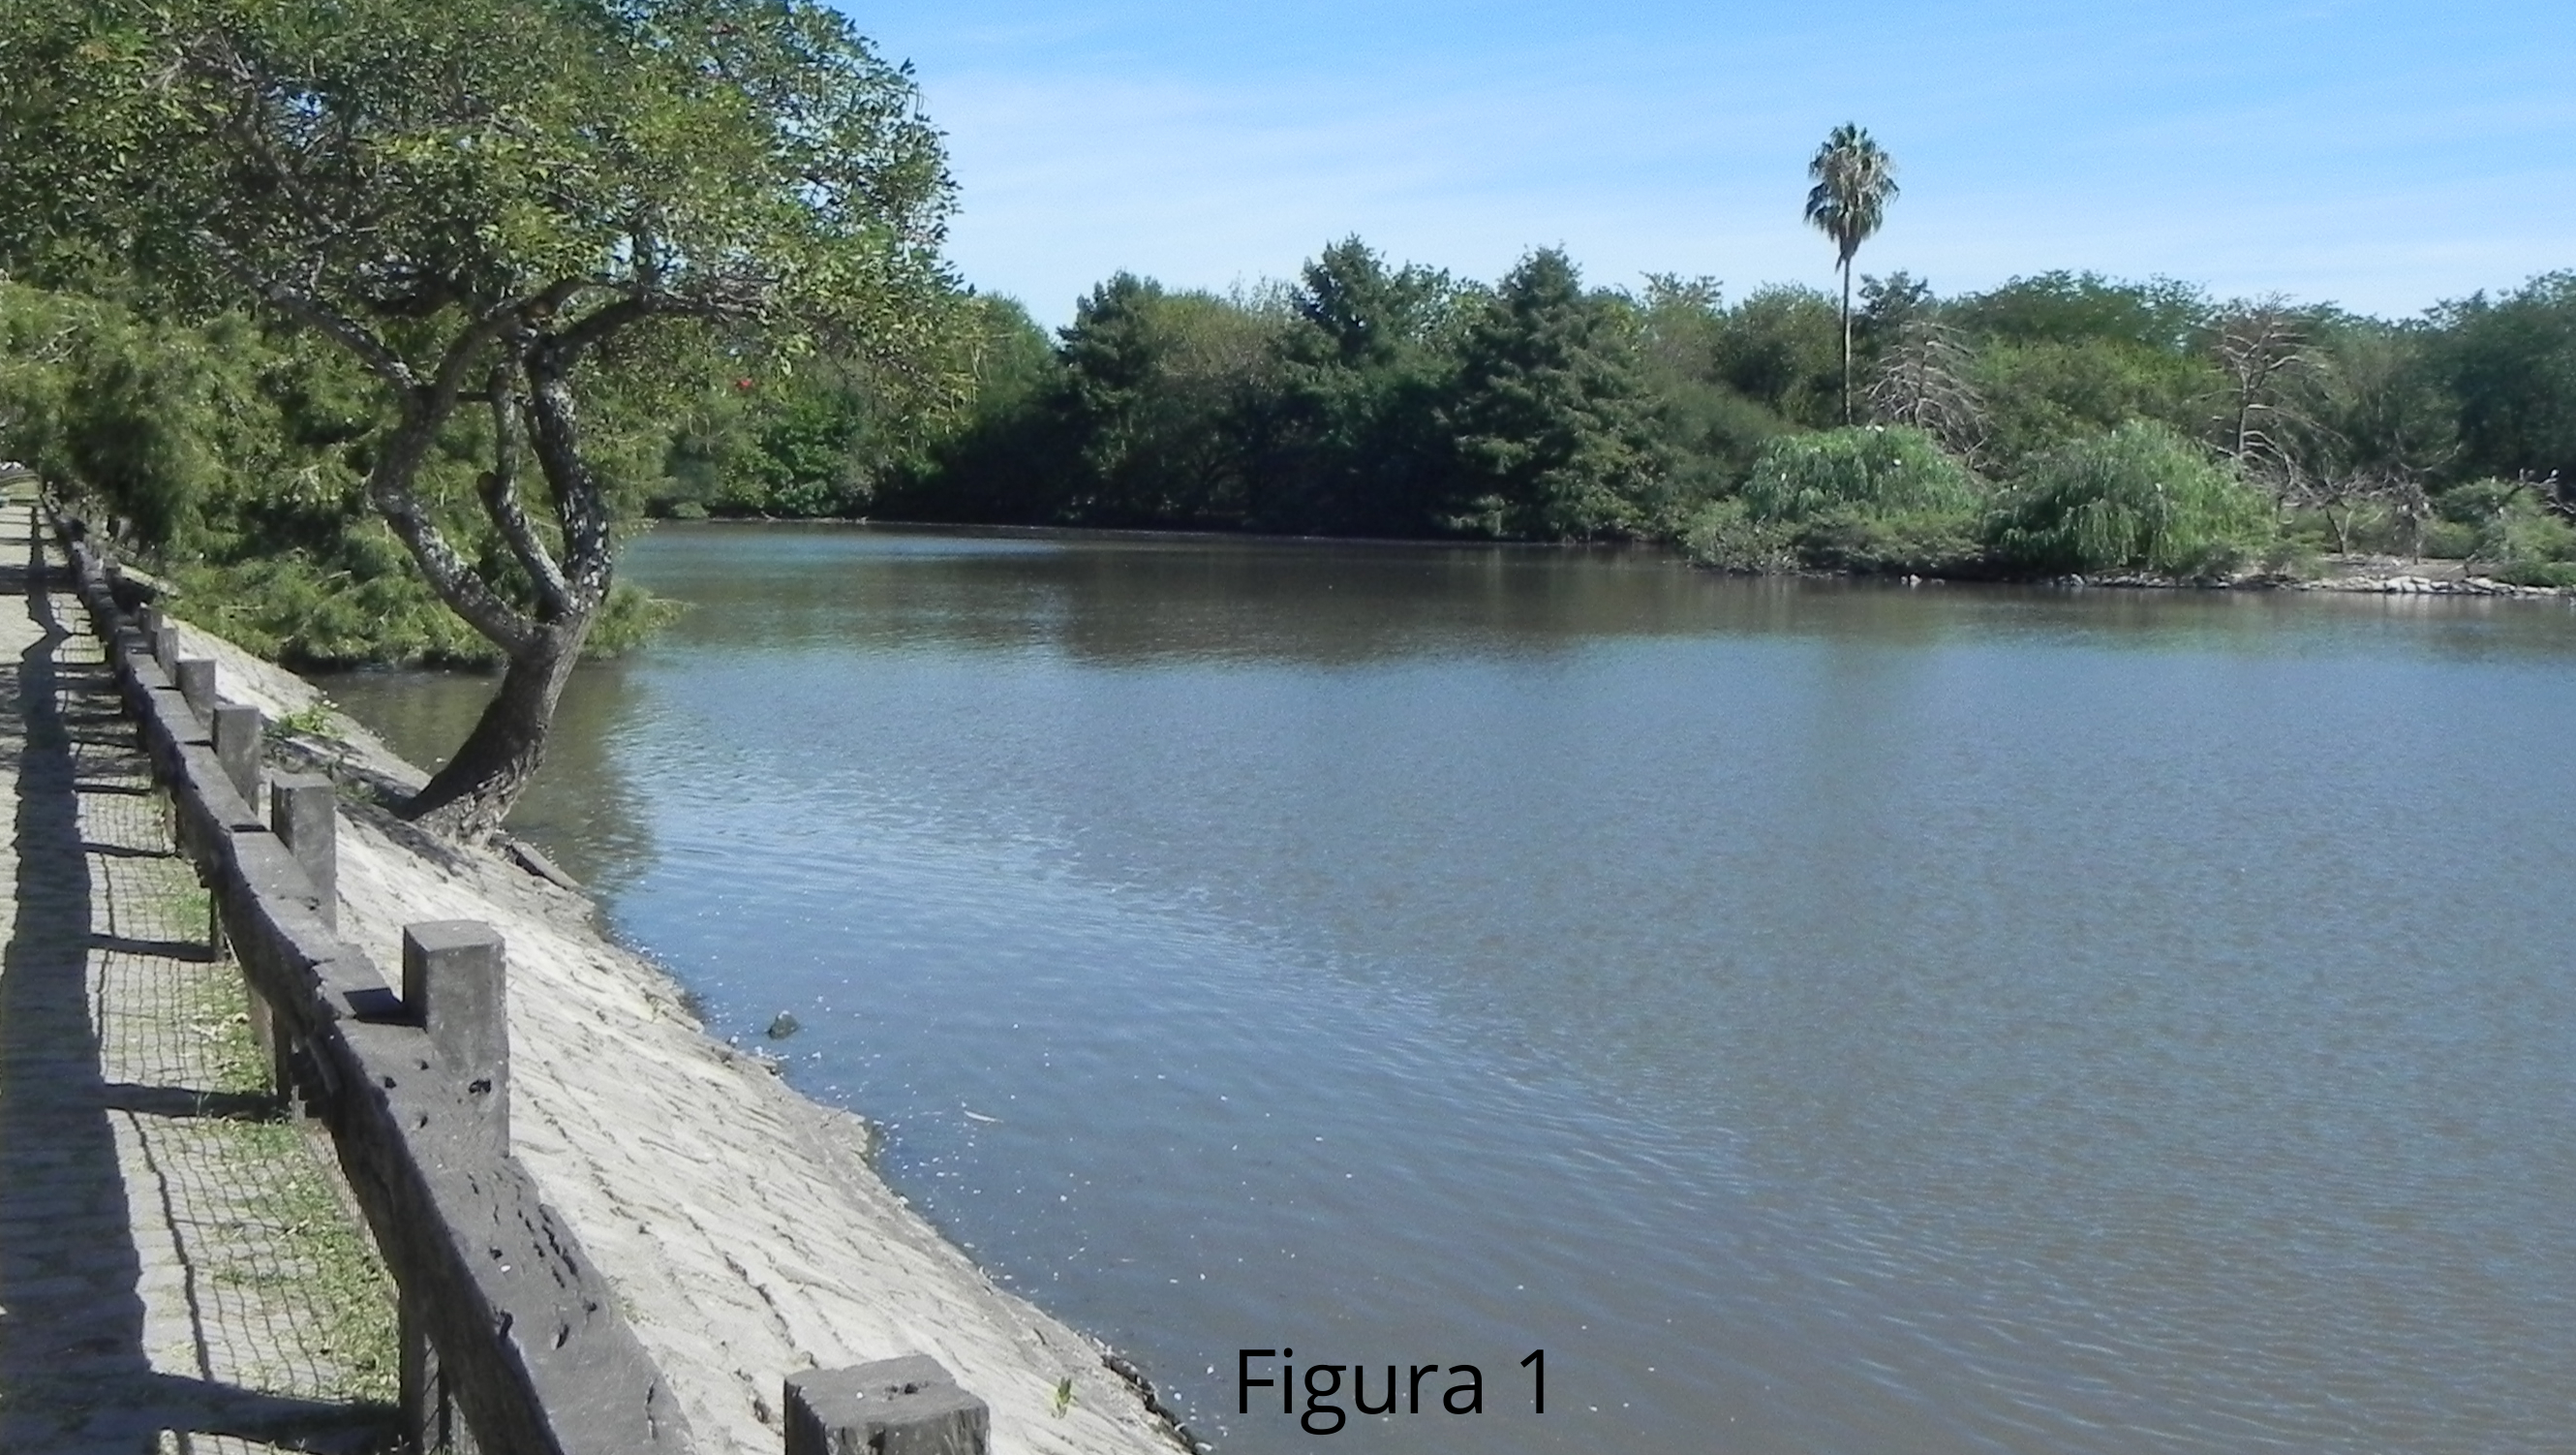
\includegraphics[width=0.9\linewidth]{lpu.jpg}
				%\end{figure}
                %\begin{figure}
                %	\vspace*{-0.90cm}
                 %   %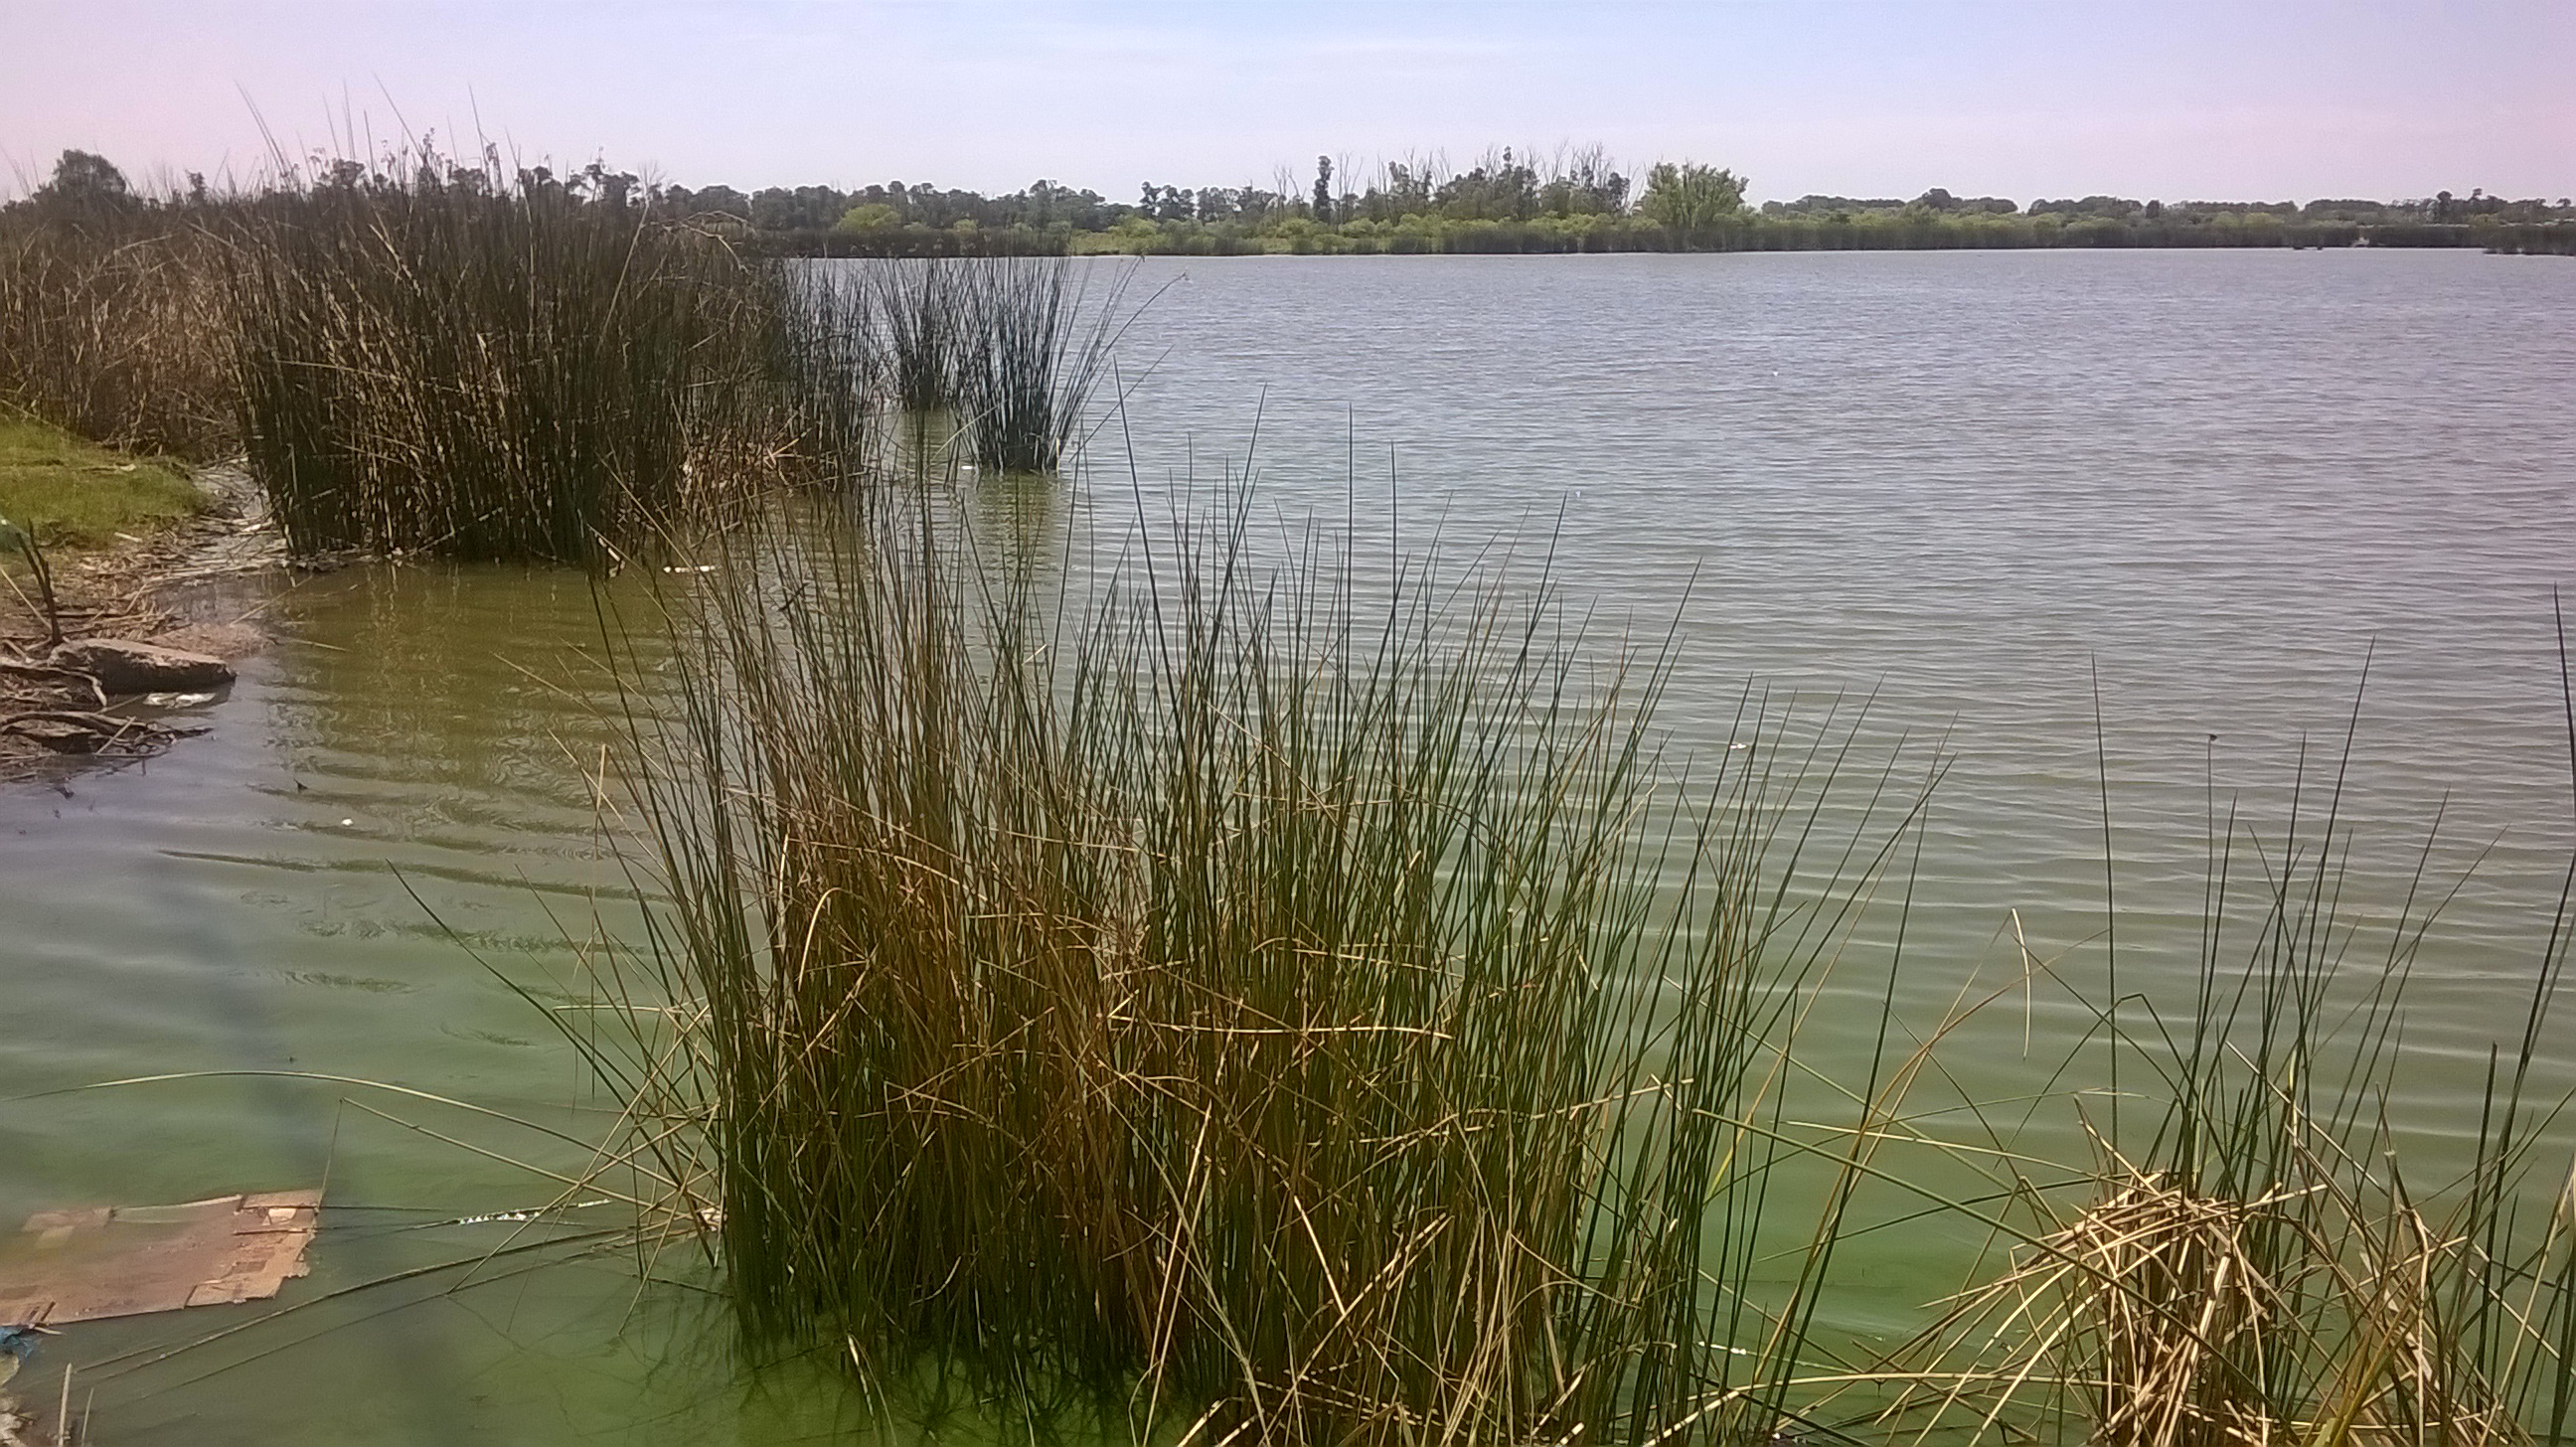
\includegraphics[width=0.9\linewidth]{lp.jpg}
				%\end{figure}
                %\end{multicols}
                
                \begin{figure}
                    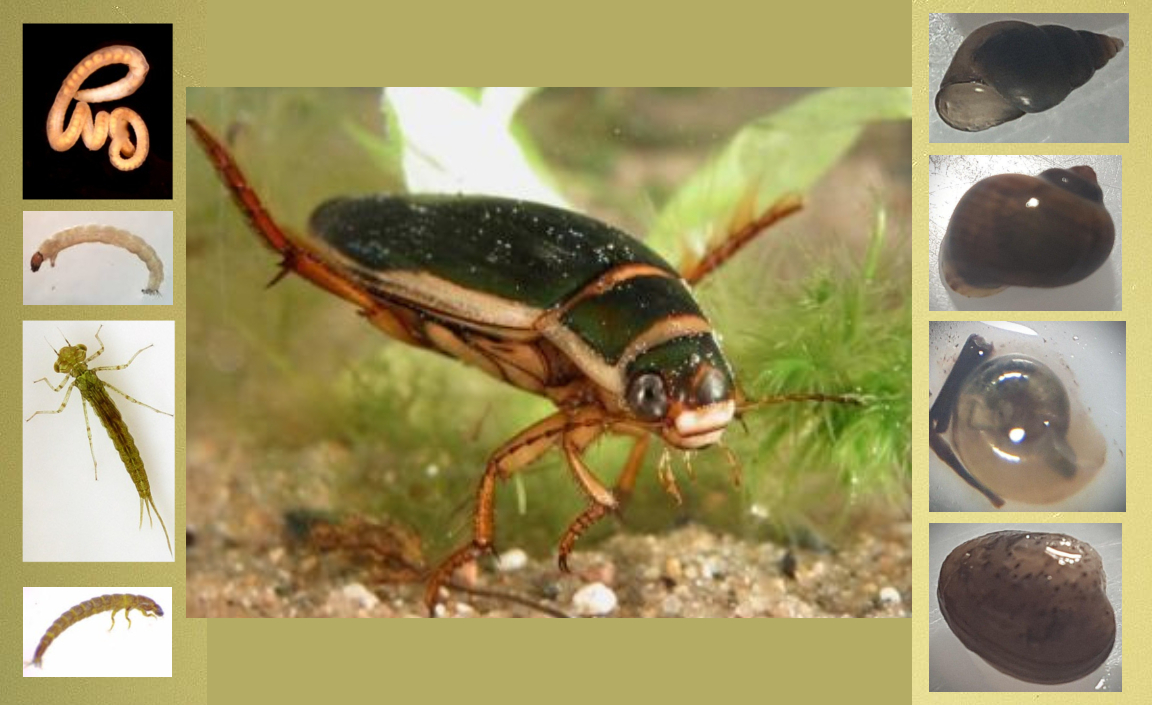
\includegraphics[width=0.45\linewidth]{popu2.jpg}
				\end{figure}
                
		\end{block}
      \end{column}
      
      \begin{column}{\sepmargin} \end{column}
      \end{columns} 
       
      \begin{columns}[t] % Split up the two columns wide column again
      
      \begin{column}{\sepmargin} \end{column}
        \begin{column}{\onecolwid} % The first column
			\begin{block}{\large Agradecimientos}
                    \begin{center}
						\begin{tabular}{SL}
							
\includegraphics[width=\linewidth]{uader.jpg}  &
							\footnotesize A la UADER por el financiamiento a través del PIDIN Res. C.S. 199/18 \textit{"Contribución al conocimiento de la ecología de dos lagunas urbanas pampeanas: laguna del parque Unzué (Gualeguaychú,Entre Ríos) y laguna Los Patos (Ensenada, Buenos Aires)"}
						\end{tabular}
					\end{center}
				\end{block}	
                \vspace*{-0.9cm}

				\begin{alertblock}{\large Información de contacto}
                \vspace*{-0.5cm}
					\begin{footnotesize}
					\begin{itemize}
						\item \href{mailto:email@meduniwien.ac.at}{laboratorioibga.fcyt@outlook.com}
						\item \href{http://cima.quimica.unlp.edu.ar//}{http://cima.quimica.unlp.edu.ar/} - \href{https://ibgafcyt.wordpress.com}{https://ibgafcyt.wordpress.com/}
					\end{itemize}
					\end{footnotesize}	
					
				\end{alertblock}
		    \end{column} % End of the first column
			\begin{column}{\sepwid}\end{column} % Empty spacer column
			\begin{column}{\onecolwid} % Begin a column 
              \begin{block}{\large Referencias}
			  \vspace*{-0.05cm}
              	\nocite{*} % Insert publications even if they are not cited in the poster
					{\footnotesize
                    	\bibliographystyle{abbrv}
						\bibliography{bibliog.bib}}
				\end{block} 
			\end{column} % End of the second column
            
			\begin{column}{\sepmargin}\end{column} % Empty spacer column
            
\end{columns} % End of all the columns in the poster


\end{frame} % End of the enclosing frame
	
\end{document}
